\documentclass[
  jou,
  floatsintext,
  longtable,
  nolmodern,
  notxfonts,
  notimes,
  colorlinks=true,linkcolor=blue,citecolor=blue,urlcolor=blue]{apa7}

\usepackage{amsmath}
\usepackage{amssymb}




\RequirePackage{longtable}
\RequirePackage{threeparttablex}

\makeatletter
\renewcommand{\paragraph}{\@startsection{paragraph}{4}{\parindent}%
	{0\baselineskip \@plus 0.2ex \@minus 0.2ex}%
	{-.5em}%
	{\normalfont\normalsize\bfseries\typesectitle}}

\renewcommand{\subparagraph}[1]{\@startsection{subparagraph}{5}{0.5em}%
	{0\baselineskip \@plus 0.2ex \@minus 0.2ex}%
	{-\z@\relax}%
	{\normalfont\normalsize\bfseries\itshape\hspace{\parindent}{#1}\textit{\addperi}}{\relax}}
\makeatother




\usepackage{longtable, booktabs, multirow, multicol, colortbl, hhline, caption, array, float, xpatch}
\usepackage{subcaption}


\renewcommand\thesubfigure{\Alph{subfigure}}
\setcounter{topnumber}{2}
\setcounter{bottomnumber}{2}
\setcounter{totalnumber}{4}
\renewcommand{\topfraction}{0.85}
\renewcommand{\bottomfraction}{0.85}
\renewcommand{\textfraction}{0.15}
\renewcommand{\floatpagefraction}{0.7}

\usepackage{tcolorbox}
\tcbuselibrary{listings,theorems, breakable, skins}
\usepackage{fontawesome5}

\definecolor{quarto-callout-color}{HTML}{909090}
\definecolor{quarto-callout-note-color}{HTML}{0758E5}
\definecolor{quarto-callout-important-color}{HTML}{CC1914}
\definecolor{quarto-callout-warning-color}{HTML}{EB9113}
\definecolor{quarto-callout-tip-color}{HTML}{00A047}
\definecolor{quarto-callout-caution-color}{HTML}{FC5300}
\definecolor{quarto-callout-color-frame}{HTML}{ACACAC}
\definecolor{quarto-callout-note-color-frame}{HTML}{4582EC}
\definecolor{quarto-callout-important-color-frame}{HTML}{D9534F}
\definecolor{quarto-callout-warning-color-frame}{HTML}{F0AD4E}
\definecolor{quarto-callout-tip-color-frame}{HTML}{02B875}
\definecolor{quarto-callout-caution-color-frame}{HTML}{FD7E14}

%\newlength\Oldarrayrulewidth
%\newlength\Oldtabcolsep


\usepackage{hyperref}




\providecommand{\tightlist}{%
  \setlength{\itemsep}{0pt}\setlength{\parskip}{0pt}}
\usepackage{longtable,booktabs,array}
\usepackage{calc} % for calculating minipage widths
% Correct order of tables after \paragraph or \subparagraph
\usepackage{etoolbox}
\makeatletter
\patchcmd\longtable{\par}{\if@noskipsec\mbox{}\fi\par}{}{}
\makeatother
% Allow footnotes in longtable head/foot
\IfFileExists{footnotehyper.sty}{\usepackage{footnotehyper}}{\usepackage{footnote}}
\makesavenoteenv{longtable}

\usepackage{graphicx}
\makeatletter
\newsavebox\pandoc@box
\newcommand*\pandocbounded[1]{% scales image to fit in text height/width
  \sbox\pandoc@box{#1}%
  \Gscale@div\@tempa{\textheight}{\dimexpr\ht\pandoc@box+\dp\pandoc@box\relax}%
  \Gscale@div\@tempb{\linewidth}{\wd\pandoc@box}%
  \ifdim\@tempb\p@<\@tempa\p@\let\@tempa\@tempb\fi% select the smaller of both
  \ifdim\@tempa\p@<\p@\scalebox{\@tempa}{\usebox\pandoc@box}%
  \else\usebox{\pandoc@box}%
  \fi%
}
% Set default figure placement to htbp
\def\fps@figure{htbp}
\makeatother


% definitions for citeproc citations
\NewDocumentCommand\citeproctext{}{}
\NewDocumentCommand\citeproc{mm}{%
  \begingroup\def\citeproctext{#2}\cite{#1}\endgroup}
\makeatletter
 % allow citations to break across lines
 \let\@cite@ofmt\@firstofone
 % avoid brackets around text for \cite:
 \def\@biblabel#1{}
 \def\@cite#1#2{{#1\if@tempswa , #2\fi}}
\makeatother
\newlength{\cslhangindent}
\setlength{\cslhangindent}{1.5em}
\newlength{\csllabelwidth}
\setlength{\csllabelwidth}{3em}
\newenvironment{CSLReferences}[2] % #1 hanging-indent, #2 entry-spacing
 {\begin{list}{}{%
  \setlength{\itemindent}{0pt}
  \setlength{\leftmargin}{0pt}
  \setlength{\parsep}{0pt}
  % turn on hanging indent if param 1 is 1
  \ifodd #1
   \setlength{\leftmargin}{\cslhangindent}
   \setlength{\itemindent}{-1\cslhangindent}
  \fi
  % set entry spacing
  \setlength{\itemsep}{#2\baselineskip}}}
 {\end{list}}
\usepackage{calc}
\newcommand{\CSLBlock}[1]{\hfill\break\parbox[t]{\linewidth}{\strut\ignorespaces#1\strut}}
\newcommand{\CSLLeftMargin}[1]{\parbox[t]{\csllabelwidth}{\strut#1\strut}}
\newcommand{\CSLRightInline}[1]{\parbox[t]{\linewidth - \csllabelwidth}{\strut#1\strut}}
\newcommand{\CSLIndent}[1]{\hspace{\cslhangindent}#1}





\usepackage{newtx}

\defaultfontfeatures{Scale=MatchLowercase}
\defaultfontfeatures[\rmfamily]{Ligatures=TeX,Scale=1}





\title{\textbf{The Mint Scale: A Fresh Validation of the Multimodal
Interoception Questionnaire and Comparison to the MAIA, BPQ and IAS}}


\shorttitle{Mint Validation}


\usepackage{etoolbox}









\authorsnames[{1,2},{1},{1}]{Dominique Makowski,Ana Neves,Giulia
Poreiro}







\authorsaffiliations{
{School of Psychology, University of Sussex},{Sussex Centre for
Consciousness Science, University of Sussex}}




\leftheader{Makowski, Neves and Poreiro}



\abstract{TO DO. }

\keywords{Interoception questionnaire, interoceptive accuracy scale,
MAIA, Mint Validation, Body Awareness}

\authornote{\par{\addORCIDlink{Dominique
Makowski}{0000-0001-5375-9967}}\par{\addORCIDlink{Ana
Neves}{0009-0006-0020-7599}}\par{\addORCIDlink{Giulia
Poreiro}{0000-0002-2343-5109}} 
\par{ }
\par{     \begin{tcolorbox}[enhanced jigsaw, colframe=quarto-callout-note-color-frame, toprule=.15mm, arc=.35mm, left=2mm, breakable, colback=white, rightrule=.15mm, bottomrule=.15mm, leftrule=.75mm, opacityback=0]

This preprint is a non-peer-reviewed work from the
\href{https://realitybending.github.io/}{\textbf{Reality Bending Lab}}.
\begin{center}

\includegraphics[width=0.2\linewidth,height=\textheight,keepaspectratio]{manuscript_files/mediabag/ReBeL_LogoOnly_hu114.png}
\end{center}

\end{tcolorbox}  Author roles were classified using the Contributor Role
Taxonomy (CRediT; https://credit.niso.org/) as follows:  Dominique
Makowski:   Conceptualization, Data curation, Formal Analysis, Funding
acquisition, Investigation, Methodology, Project
administration, Resources, Software, Supervision, Validation, Visualization, Writing
-- original draft; Ana Neves:   Investigation, Methodology, Project
administration, Supervision, Writing -- original draft, Writing --
review \& editing; Giulia Poreiro:   Investigation, Methodology, Writing
-- original draft, Writing -- review \& editing}
\par{Correspondence concerning this article should be addressed
to Dominique
Makowski, Email: \href{mailto:D.Makowski@sussex.ac.uk}{D.Makowski@sussex.ac.uk}}
}

\usepackage{pbalance}
% \usepackage{float}
\makeatletter
\let\oldtpt\ThreePartTable
\let\endoldtpt\endThreePartTable
\def\ThreePartTable{\@ifnextchar[\ThreePartTable@i \ThreePartTable@ii}
\def\ThreePartTable@i[#1]{\begin{figure}[!htbp]
\onecolumn
\begin{minipage}{0.485\textwidth}
\oldtpt[#1]
}
\def\ThreePartTable@ii{\begin{figure}[!htbp]
\onecolumn
\begin{minipage}{0.48\textwidth}
\oldtpt
}
\def\endThreePartTable{
\endoldtpt
\end{minipage}
\twocolumn
\end{figure}}
\makeatother


\makeatletter
\let\endoldlt\endlongtable		
\def\endlongtable{
\hline
\endoldlt}
\makeatother

\newenvironment{twocolumntable}% environment name
{% begin code
\begin{table*}[!htbp]%
\onecolumn%
}%
{%
\twocolumn%
\end{table*}%
}% end code

\urlstyle{same}



\makeatletter
\@ifpackageloaded{tcolorbox}{}{\usepackage[skins,breakable]{tcolorbox}}
\@ifpackageloaded{fontawesome5}{}{\usepackage{fontawesome5}}
\definecolor{quarto-callout-color}{HTML}{909090}
\definecolor{quarto-callout-note-color}{HTML}{0758E5}
\definecolor{quarto-callout-important-color}{HTML}{CC1914}
\definecolor{quarto-callout-warning-color}{HTML}{EB9113}
\definecolor{quarto-callout-tip-color}{HTML}{00A047}
\definecolor{quarto-callout-caution-color}{HTML}{FC5300}
\definecolor{quarto-callout-color-frame}{HTML}{acacac}
\definecolor{quarto-callout-note-color-frame}{HTML}{4582ec}
\definecolor{quarto-callout-important-color-frame}{HTML}{d9534f}
\definecolor{quarto-callout-warning-color-frame}{HTML}{f0ad4e}
\definecolor{quarto-callout-tip-color-frame}{HTML}{02b875}
\definecolor{quarto-callout-caution-color-frame}{HTML}{fd7e14}
\makeatother
\makeatletter
\@ifpackageloaded{caption}{}{\usepackage{caption}}
\AtBeginDocument{%
\ifdefined\contentsname
  \renewcommand*\contentsname{Table of contents}
\else
  \newcommand\contentsname{Table of contents}
\fi
\ifdefined\listfigurename
  \renewcommand*\listfigurename{List of Figures}
\else
  \newcommand\listfigurename{List of Figures}
\fi
\ifdefined\listtablename
  \renewcommand*\listtablename{List of Tables}
\else
  \newcommand\listtablename{List of Tables}
\fi
\ifdefined\figurename
  \renewcommand*\figurename{Figure}
\else
  \newcommand\figurename{Figure}
\fi
\ifdefined\tablename
  \renewcommand*\tablename{Table}
\else
  \newcommand\tablename{Table}
\fi
}
\@ifpackageloaded{float}{}{\usepackage{float}}
\floatstyle{ruled}
\@ifundefined{c@chapter}{\newfloat{codelisting}{h}{lop}}{\newfloat{codelisting}{h}{lop}[chapter]}
\floatname{codelisting}{Listing}
\newcommand*\listoflistings{\listof{codelisting}{List of Listings}}
\makeatother
\makeatletter
\makeatother
\makeatletter
\@ifpackageloaded{caption}{}{\usepackage{caption}}
\@ifpackageloaded{subcaption}{}{\usepackage{subcaption}}
\makeatother

% From https://tex.stackexchange.com/a/645996/211326
%%% apa7 doesn't want to add appendix section titles in the toc
%%% let's make it do it
\makeatletter
\xpatchcmd{\appendix}
  {\par}
  {\addcontentsline{toc}{section}{\@currentlabelname}\par}
  {}{}
\makeatother

%% Disable longtable counter
%% https://tex.stackexchange.com/a/248395/211326

\usepackage{etoolbox}

\makeatletter
\patchcmd{\LT@caption}
  {\bgroup}
  {\bgroup\global\LTpatch@captiontrue}
  {}{}
\patchcmd{\longtable}
  {\par}
  {\par\global\LTpatch@captionfalse}
  {}{}
\apptocmd{\endlongtable}
  {\ifLTpatch@caption\else\addtocounter{table}{-1}\fi}
  {}{}
\newif\ifLTpatch@caption
\makeatother

\begin{document}

\maketitle



\setcounter{secnumdepth}{-\maxdimen} % remove section numbering

\setlength\LTleft{0pt}




\section{Introduction}\label{introduction}

TODO: write general intro.

Main issues in existing questionnaires: - Either heavily based on
theories (e.g., focusing on a specific dimensions), despite shaky
evidence for said-theories - Do not control for context (which leads to
variability in interpretation and occurence) - Often quite narrow in the
modalities covered

\section{Study 1: Item Selection}\label{study-1-item-selection}

TODO: write intro.

Goal of study 1: to generate a lot of items, analyze its structure and
reduce them to a balanced set of items.

\subsection{Methods}\label{methods}

\subsubsection{Participants}\label{participants}

We recruited 760 English-speaking participants using
Prolific\textcopyright. We excluded 191 for failing at least one
attention check, and 10 based on measures significantly related to the
probability of failing attention checks (namely, the multivariate
distance obtained with the OPTICS algorithm,
\citeproc{ref-theriault2024check}{Thériault et al., 2024}). The final
sample includes 559 participants (age = 37.0 \(\pm\) 12.2 {[}18, 77{]};
50.8\% women; Country of residence: 63.86\% UK, 26.65\% USA). This study
was approved by the University of Sussex' Ethics Committee
(\textbf{NUMBER}).

\subsubsection{Item Generation}\label{item-generation}

Based on the two goals outlined for this scale, namely to include
different interoceptive modalities, and to explicitly state the context
of the interoceptive experience (e.g., whether negative or positive), we
generated items in a systematic way following a combinatorial approach,
where each item's category was a combination of a specific modality and
context (Figure~\ref{fig-one}).

\begin{figure*}[!htbp]

{\caption{{The conceptual grid used to generate the 120 initial items
(top-left). Each item belong both to an interoceptive modalitiy and a
facet, with the number of each item per category indicated in the
circles. The askterisk denotes the additional presence of an attention
check item in that category. In the experiment, these items were
presented on different pages grouped either by modality (bottom-left),
by facet (top-right), or entirely randomly. The Correlation Similarity
(bottom-right) analysis suggested that the correlation matrix obtained
from the participants assigned to the random-grouping condition was
slightly more similar (but non-significantly) to the one obtained in the
modality-grouping condition, suggesting that 1) the scale's structure is
robust to different presentation conditions; 2) modality-grouping might
tend to facilitate the emergence of the underlying item structure (and
thus be interpreted as being more natural).}{\label{fig-one}}}}

\begin{center}
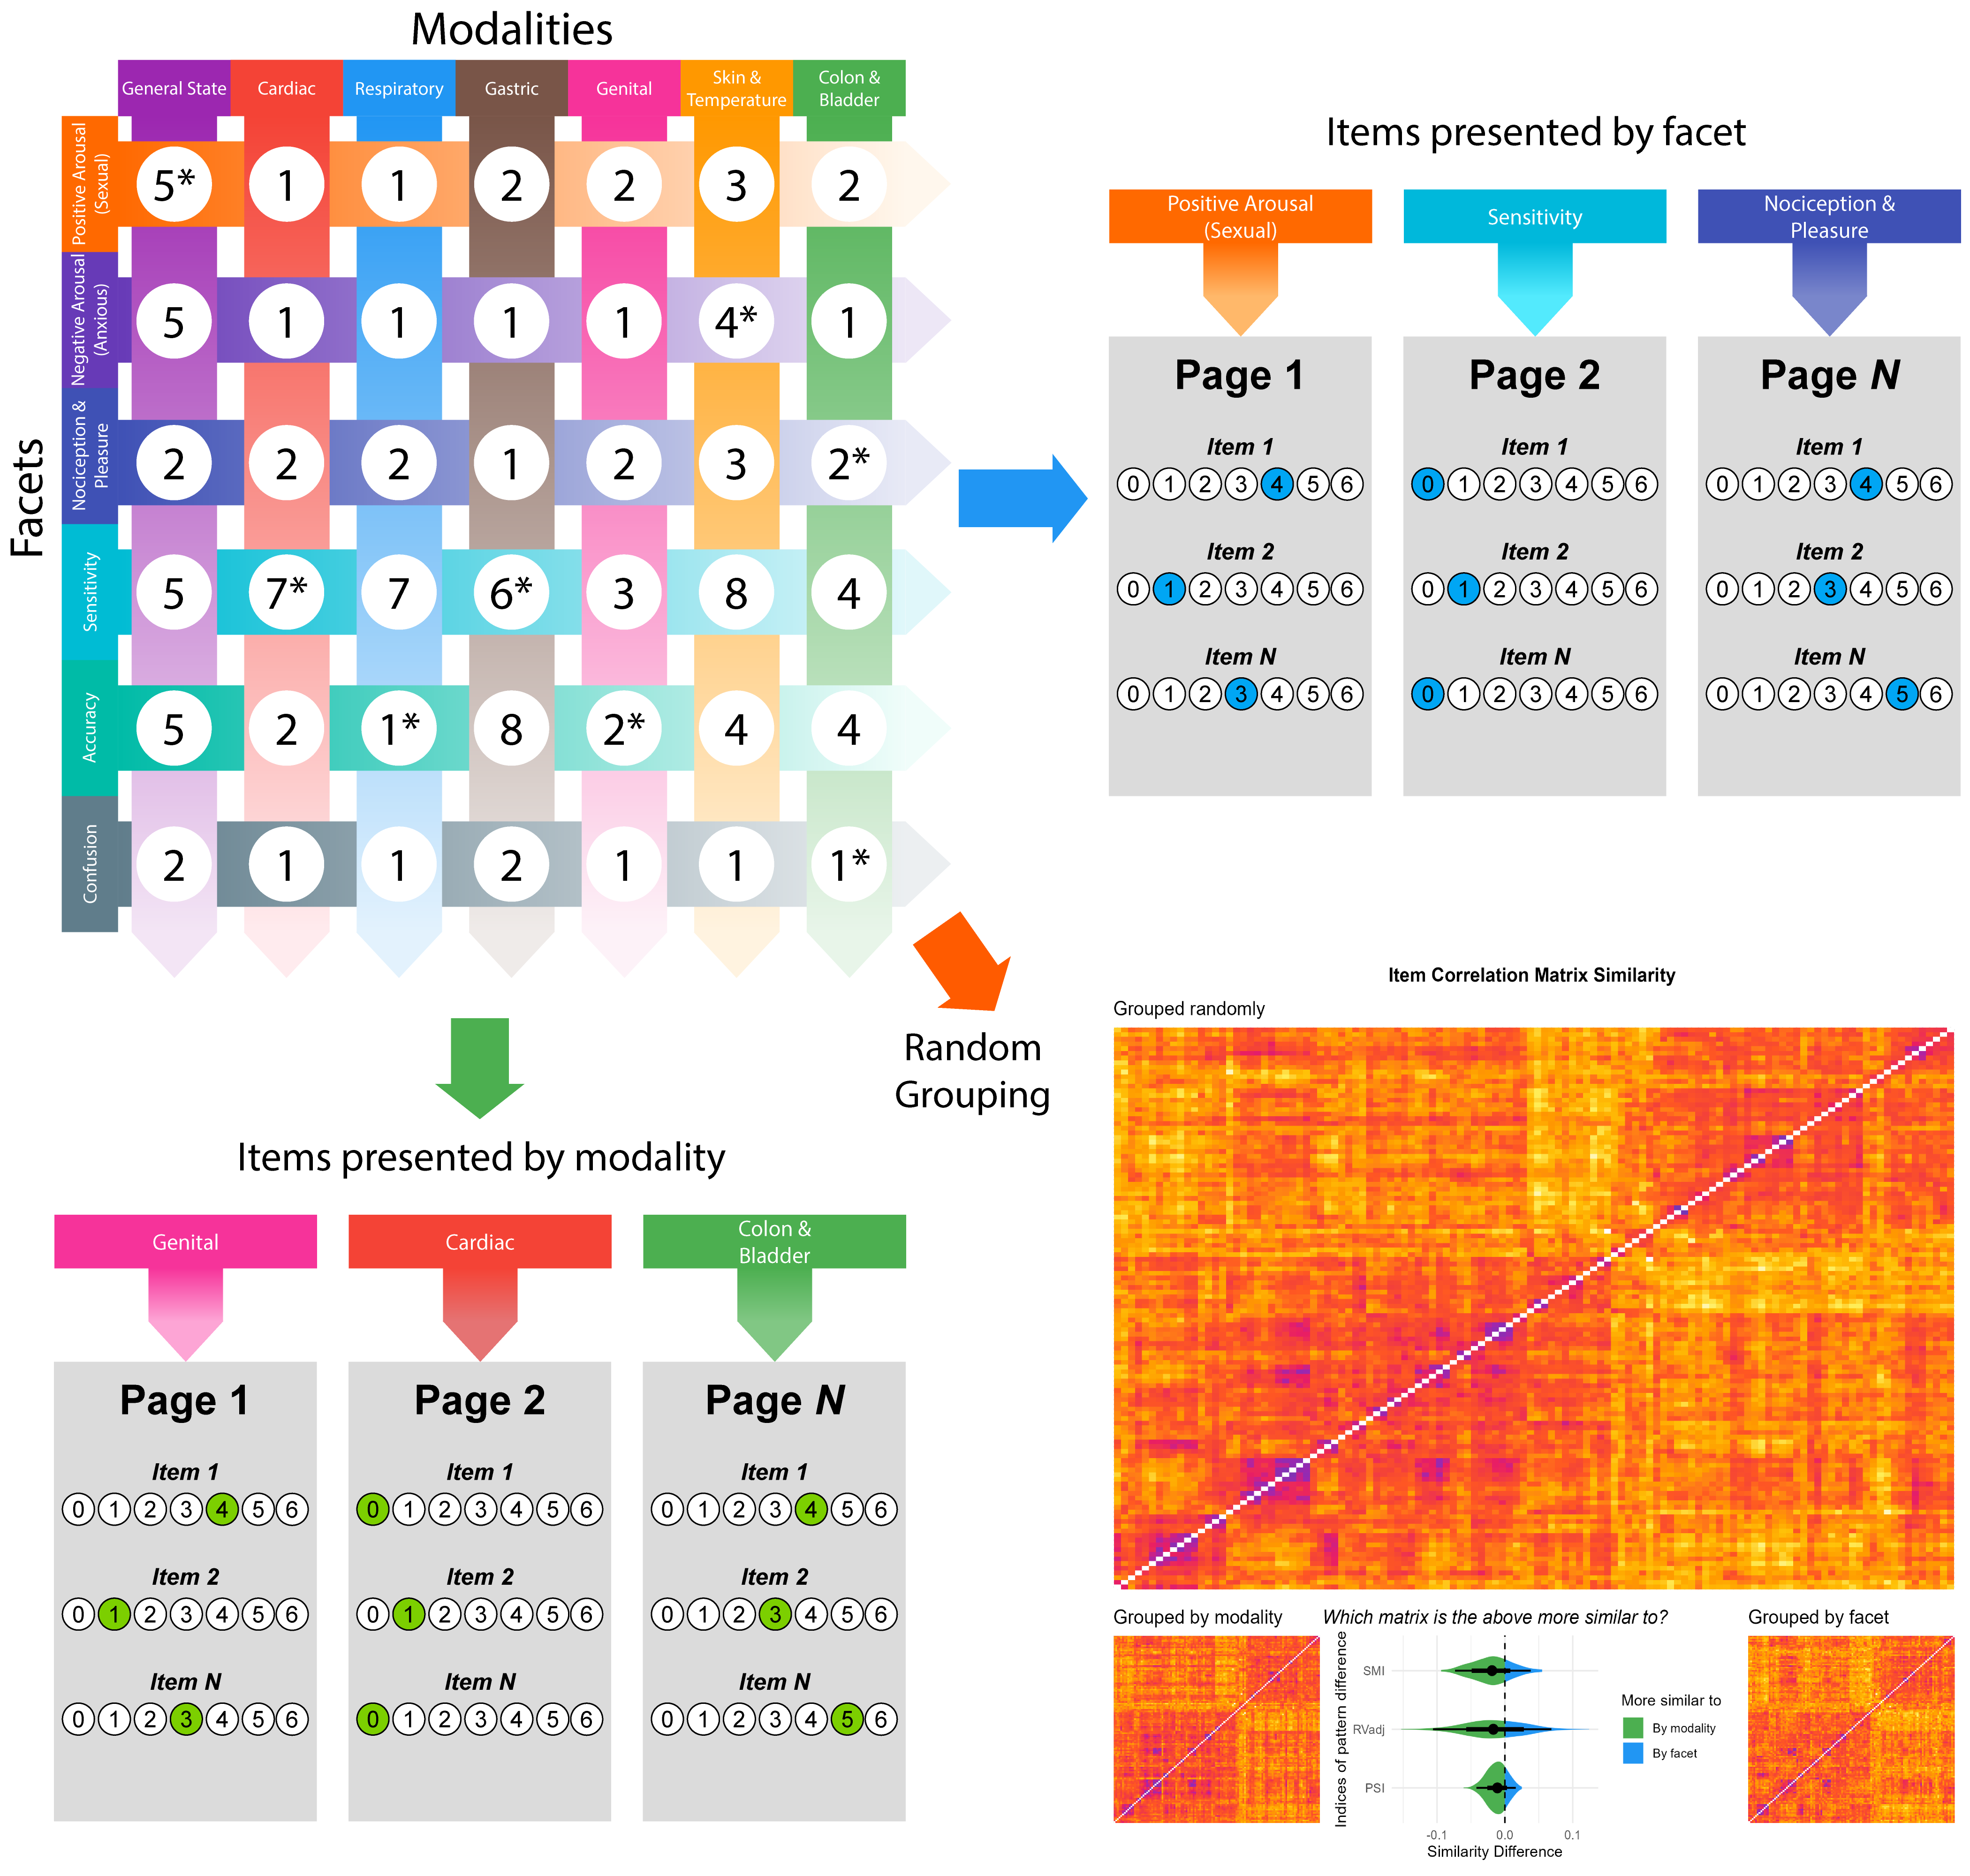
\includegraphics[width=1\linewidth,height=\textheight,keepaspectratio]{../study1/analysis/figures/figure1.png}
\end{center}

\end{figure*}

We firstly identified 7 ``modalities'' (cardiac, respiratory, gastric,
genital, skin \& temperature, bladder \& colon, and a ``general state''
category corresponding to a holistic and general awareness of an
interoceptive state or dimension). Through iterative refinement (e.g.,
splitting or merging different categories together), we then settled on
6 ``facets'', which encompass both \emph{contexts} of experience
(negative and positive arousal, namely anxious and sexual states), and
potential distinct \emph{mechanisms} (nociception \& pleasure,
sensitivity, accuracy, and confusion).

Using this orthogonal 7x6 modality/facet grid as a conceptual
scaffolding, we generated 120 initial items, striving for a balanced
number of items with consistent phrasing within modalities and
facets\footnote{The initial item list at
  \href{https://realitybending.github.io/InteroceptionScale/study1/analysis/2_analysis.html}{realitybending.github.io/InteroceptionScale/study1/analysis/2\_analysis.html}}.
We additionally crafted 8 ``attention check'' items blending in (and
distributed across) each category.

\subsubsection{Procedure}\label{procedure}

To avoid presenting all the 120 items on a single long and discouraging
page, we split them into different pages. Participants were randomly
assigned to one of three conditions, driving how items were grouped on
the same page: 1) items grouped by modality (i.e., all cardiac items on
the first page, all colon \& bladder items on the second, etc.), 2)
items grouped by facet, or 3) items presented fully randomly (but
balanced randomly across 6 pages). The order of the item on any given
page and the order of the modalities/facets were randomized. Each
participant completed the full set of 120 items, with the attention
check items interspersed throughout. The online experiment was
implemented using JsPsych (\citeproc{ref-de2015jspsych}{De Leeuw,
2015}), and item responses were recorded using 7-points Likert scales (0
= Disagree, 6 = Agree).

\subsubsection{Data Analysis}\label{data-analysis}

In order to test whether the grouping condition had an effect on the
structure (i.e., how items relate to one-another), we compared the
correlation matrix obtained in the random condition to the ones obtained
in the modality and facet conditions, focusing on 3 indices of
correlation matrix similarity - the Procrustes Similarity Index (PSI,
\citeproc{ref-sibson1978studies}{Sibson, 1978}), the Adjusted RV (Rvadj,
\citeproc{ref-mayer2011exploratory}{Mayer et al., 2011}), and the
Similarity of Matrices Index (SMI,
\citeproc{ref-indahl2018similarity}{Indahl et al., 2018}). For each
index, we bootstrapped the difference between the similarity with the
facet and modality conditions to test whether the correlation matrix in
the random-grouping condition is significantly more similar to any of
the two other conditions.

Items deemed ``redundant'' (which can distort the item structure
estimation by introducing multicollinearity or local dependencies) will
be identified (using the recommended threshold of 0.25) using Unique
Variable Analysis (UVA, \citeproc{ref-christensen2023unique}{Christensen
et al., 2023}), a novel and principled method derived from network
psychometrics.

The structure of the items will be analyzed using the recently-developed
Exploratory Graph Analysis (EGA, \citeproc{ref-golino2017exploratory}{H.
F. Golino \& Epskamp, 2017}) framework, which allows to jointly estimate
the number of dimensions (i.e., clusters of items), the structure, as
well as its stability using bootstrapping
(\citeproc{ref-golino2020investigating}{H. Golino et al., 2020}). At a
fundamental level, EGA conceptualizes variables as nodes in a network,
with connections (edges) reflecting associations between them. Evidence
has underlined its suitability as an alternative to traditional factor
analysis, addressing some of its limitations such as the assumption of a
``latent'' source of variability, issues in estimation of the optimal
factor numbers, and poor performance in complex population structures,
while remaining comparable and interpretable
(\citeproc{ref-christensen2021equivalency}{Christensen \& Golino, 2021};
\citeproc{ref-jimenez2023dimensionality}{Jiménez et al., 2023}). In
particular, nodes communities (i.e., clusters of items) can be in
practice interpreted as distinct ``dimensions'', similarly to
traditional latent factors - but without explicitly assuming their
existence (\citeproc{ref-christensen2021equivalency}{Christensen \&
Golino, 2021}).

After removing redundant items using UVA, we will iteratively fit
hierarchical EGA models (which additionally estimates higher-order
``meta'' clusters) using ``glasso'' {[}\textbf{REF}{]} and the
``leiden'' algorithm {[}\textbf{REF}{]} for community detection,
refining the item pool at each step. We will start by removing items
with a low (\textless{} 80\%) cluster stability (i.e., volatile items
which jump between clusters across bootstrapped samples), followed by
odd items belonging to no clusters or pairs of items (i.e., we keep
items belonging to clusters of more than 2 items). Finally, for each
lower-level cluster, we will select the 3 items with the highest node
centrality (i.e., the highest loading in the cluster).

\subsection{Results}\label{results}

The correlation matrix similarity analysis yielded no significant
differences between the similarity of the random-grouping condition with
the modality-grouping and facet-grouping conditions
(\(PSI_{\text{Random vs. Facet}} = 0.81\),
\(PSI_{\text{Random vs. Modality}} = 0.82\), \(p = .45\);
\(RVadj_{\text{Random vs. Facet}} = 0.77\),
\(RVadj_{\text{Random vs. Modality}} = 0.78\), \(p = .74\);
\(SMI_{\text{Random vs. Facet}} = 0.49\),
\(SMI_{\text{Random vs. Modality}} = 0.51\), \(p = .52\)).

From the 120 initial items, UVA flagged 4 redundant items that we
removed. We then removed 40 items that showed low cluster stability, and
9 items that were part of clusters with less than 3 items. Finally, We
kept the 3 items with the highest loading in their lower-level structure
(removing 13 items in the process), resulting in 54 items in the final
item pool.

The final hierarchical EGA model (Generalized Total Entropy Fit Index =
-119.18) - in which all 54 items yielded a high cluster stability
(\textgreater{} 90\%) suggested 3 metaclusters and 15 lower-level
clusters (each containing 3 items): ``Interoceptive Deficits''
(containing 5 clusters: \emph{Urointestinal Inaccuracy} - UrIn;
\emph{Cardiorespiratory Confusion} - CaCo; \emph{Cardiorespiratory
Noticing} - CaNo; \emph{Olfactory Compensation} - Olfa; \emph{Satiety
Noticing} - Sati), ``Interoceptive Awareness'' (containing 7 clusters:
\emph{Sexual Arousal Awareness} - SexA; \emph{Sexual Arousal
Sensitivity} - SexS; \emph{Sexual Organs Sensitivity} - SexO;
\emph{Urointestinal Sensitivity} - UrSe; \emph{Relaxation Awareness} -
RelA; \emph{State Specificity} - StaS; \emph{Expulsion Accuracy} -
ExAc), and ``Interoceptive Sensitivity'' (containing 6 clusters:
\emph{Cardioception} - Card; \emph{Respiroception} - Resp;
\emph{Signalling} - Sign; \emph{Gastroception} - Gast; \emph{Dermal
Hypersensitivity} - Derm; \emph{Sexual Arousal Changes} - SexC).

To further reduce and balance the remaining items, we collectively
decided on removing the lower-level clusters \emph{Sexual Arousal
Awareness} (too general and overlapping with the other more specific
sex-related items), \emph{Signalling} (which items started with ``when
something important is happening in my life'', which meaning we deemed
too much open to interpretation), and \emph{Sexual Arousal Changes} (low
fit with the other modality-focused clusters of its group). The final
set included 45 items.

\subsection{Discussion}\label{discussion}

Possible (although not at all significant) bias consistent across
indices in favour of a greater similarity with the modality-grouping
condition.

\section{Study 2: Validation}\label{study-2-validation}

TODO: write intro. Goal of study 2: to validate the Mint scale against
other interoception scales.

\subsection{Methods}\label{methods-1}

\subsubsection{Participants}\label{participants-1}

We recruited 921 English-speaking participants via
Prolific\textcopyright and SONA, from which 118 were excluded for
failing at least one attention check and 6 based on multivariate
distance (using the same procedure as for study 1). 60 participants were
further excluded due to missing data following a technical error. The
final sample includes 737 participants (age = 36.8 \(\pm\) 14.7 {[}18,
87{]}; 57.3\% women; Country of residence: 75.17\% United Kingdom,
24.83\% other). This study was approved by the University of Sussex'
Ethics Committee (\textbf{NUMBER}).

\subsubsection{Procedure}\label{procedure-1}

The experiment included the following questionnaires.

\paragraph{Interoception
Questionnaires.}\label{interoception-questionnaires}

\subparagraph{The Multimodal Interoception Questionnaire
(Mint).}\label{the-multimodal-interoception-questionnaire-mint}

The 45 items of the Mint scale were presented in a random order, with
the same 7-point Likert scale as in study 1 (0 = Disagree, 6 = Agree).

\subparagraph{Multidimensional Assessment of Interoceptive Awareness
(MAIA).}\label{multidimensional-assessment-of-interoceptive-awareness-maia}

The X items of the MAIA\ldots{}

\subparagraph{The Body Perception Questionnaire
(BPQ).}\label{the-body-perception-questionnaire-bpq}

\textbf{TODO}

\subparagraph{The Interoceptive Awareness Scale
(IAS).}\label{the-interoceptive-awareness-scale-ias}

\textbf{TODO}

\paragraph{Emotions and Cognition.}\label{emotions-and-cognition}

\subparagraph{Toronto Alexithymia Scale
(TAS-20).}\label{toronto-alexithymia-scale-tas-20}

\textbf{TODO}

\subparagraph{Emotion Reactivity Scale
(ERS).}\label{emotion-reactivity-scale-ers}

\textbf{TODO}

\subparagraph{Cognitive Emotion Regulation Questionnaire
(CERQ).}\label{cognitive-emotion-regulation-questionnaire-cerq}

\textbf{TODO}

\subparagraph{TODO (CEFSA).}\label{todo-cefsa}

\textbf{TODO}

\subparagraph{Primal World Beliefs
(PI-18).}\label{primal-world-beliefs-pi-18}

\textbf{TODO}

\paragraph{Health and Wellbeing.}\label{health-and-wellbeing}

\subparagraph{Life Satisfaction, Depression and Anxiety
(PHQ-4).}\label{life-satisfaction-depression-and-anxiety-phq-4}

\textbf{TODO}

\subparagraph{Mental Health.}\label{mental-health}

Participants were asked to self-report any current, medically diagnosed
psychiatric disorders using a checklist based on DSM-5 categories. If
one or more conditions were endorsed, participants were asked to
indicate any current treatments, including pharmacological (e.g.,
antidepressants, anxiolytics, antipsychotics, mood stabilizers),
psychological (e.g., psychotherapy, mindfulness), or lifestyle
interventions. Binary variables (0 = absent, 1 = present) were created
to identify participants reporting mood disorders (MDD, GAD, Bipolar
Disorder; with a stricter subgroup of participants undergoing a pharma-
or psychological treatment), anxiety-centred disorders (GAD, Panic
Disorder, Social Anxiety Disorder, Specific Phobias), eating disorders,
addiction-related disorders, borderline personality disorder, autism
spectrum disorder (ASD), and ADHD.

\subparagraph{Somatic Health.}\label{somatic-health}

Participants were asked to select somatic symptoms or conditions they
experienced from a list of 36 options. To facilitate mechanistic
interpretation and reduce redundancy, answers were grouped into four
non-overlapping clusters based on shared physiological pathways and
known etiological mechanisms. The \emph{Afferent Sensitivity} cluster
included conditions associated with heightened interoceptive awareness
and neurogenic excitability, such as migraine, neuropathy, dizziness,
nausea, muscle tension, epilepsy, and frequent urination. The
\emph{Central Sensitization} cluster comprised syndromes characterized
by chronic pain and fatigue, likely reflecting central amplification of
sensory signals and HPA-axis dysregulation, such as fibromyalgia,
chronic fatigue syndrome, chronic pain, back pain, pelvic pain,
irritable bowel syndrome (IBS). The \emph{Autonomic Dysfunction} cluster
captured disorders linked to dysregulation of the autonomic and
cardiopulmonary systems, including joint hypermobility, cardiac
arrhythmia, chest pain, shortness of breath, hypo-/hypertension, sleep
apnea, chronic obstructive pulmonary disease (COPD), and chronic
bronchitis. Finally, the \emph{Immune-Inflammatory} cluster encompassed
conditions associated with immune dysregulation, barrier dysfunction,
and gut-brain axis disturbance, such as eczema, psoriasis, skin rashes,
asthma, celiac disease, gluten and lactose sensitivity, inflammatory
bowel diseases (Crohn's disease and ulcerative colitis),
gastroesophageal reflux disease (GERD), multiple sclerosis, and
Sjögren's syndrome. We scored each cluster as a binary variable based on
whether the participant selected at least one symptom from that cluster.

\paragraph{Lifestyle.}\label{lifestyle}

\textbf{TODO}

Physical activity.

Wearables.

\paragraph{Randomization.}\label{randomization}

In order to avoid the repetition of similar types of questions and and
balance longer and shorter questionnaires, we partitioned them into
three groups (and randomized their order within them): (1) interoception
questionnaires (MAIA, IAS, BPQ), (2) emotions (TAS, CERQ, ERS, PI-18),
and (3) pathology (somatic health, mental health, LS + PHQ-4, CEFSA).
After completing demographic questions, participants always started with
the Mint scale, and each following interoception questionnaire was
interspersed with two questionnaires from the emotions and pathology
groups. In order to make the experiment more enjoyable, the experiment
ended with a radar chart summarizing the participants' responses to the
Mint scale\footnote{The experiment can be tested by following the link
  on https://github.com/RealityBending/InteroceptionScale}.

\subsubsection{Data Analysis}\label{data-analysis-1}

We will start by confirming and further refining the structure of the
Mint scale using the same EGA model as in Study 1. The convergent
validity of the final set of items will be assessed by computing the
correlations between the Mint scale and the other interoception
questionnaires (MAIA, BPQ, IAS). Then, we will test the predictive power
of the Mint scale (relative to the other interoception questionnaires)
on various measures. We will start by fitting regression (linear for
continuous measures - e.g., depression score - and logistic for binary

\begin{figure*}[!htbp]

{\caption{{TODO.}{\label{fig-two}}}}

\begin{center}
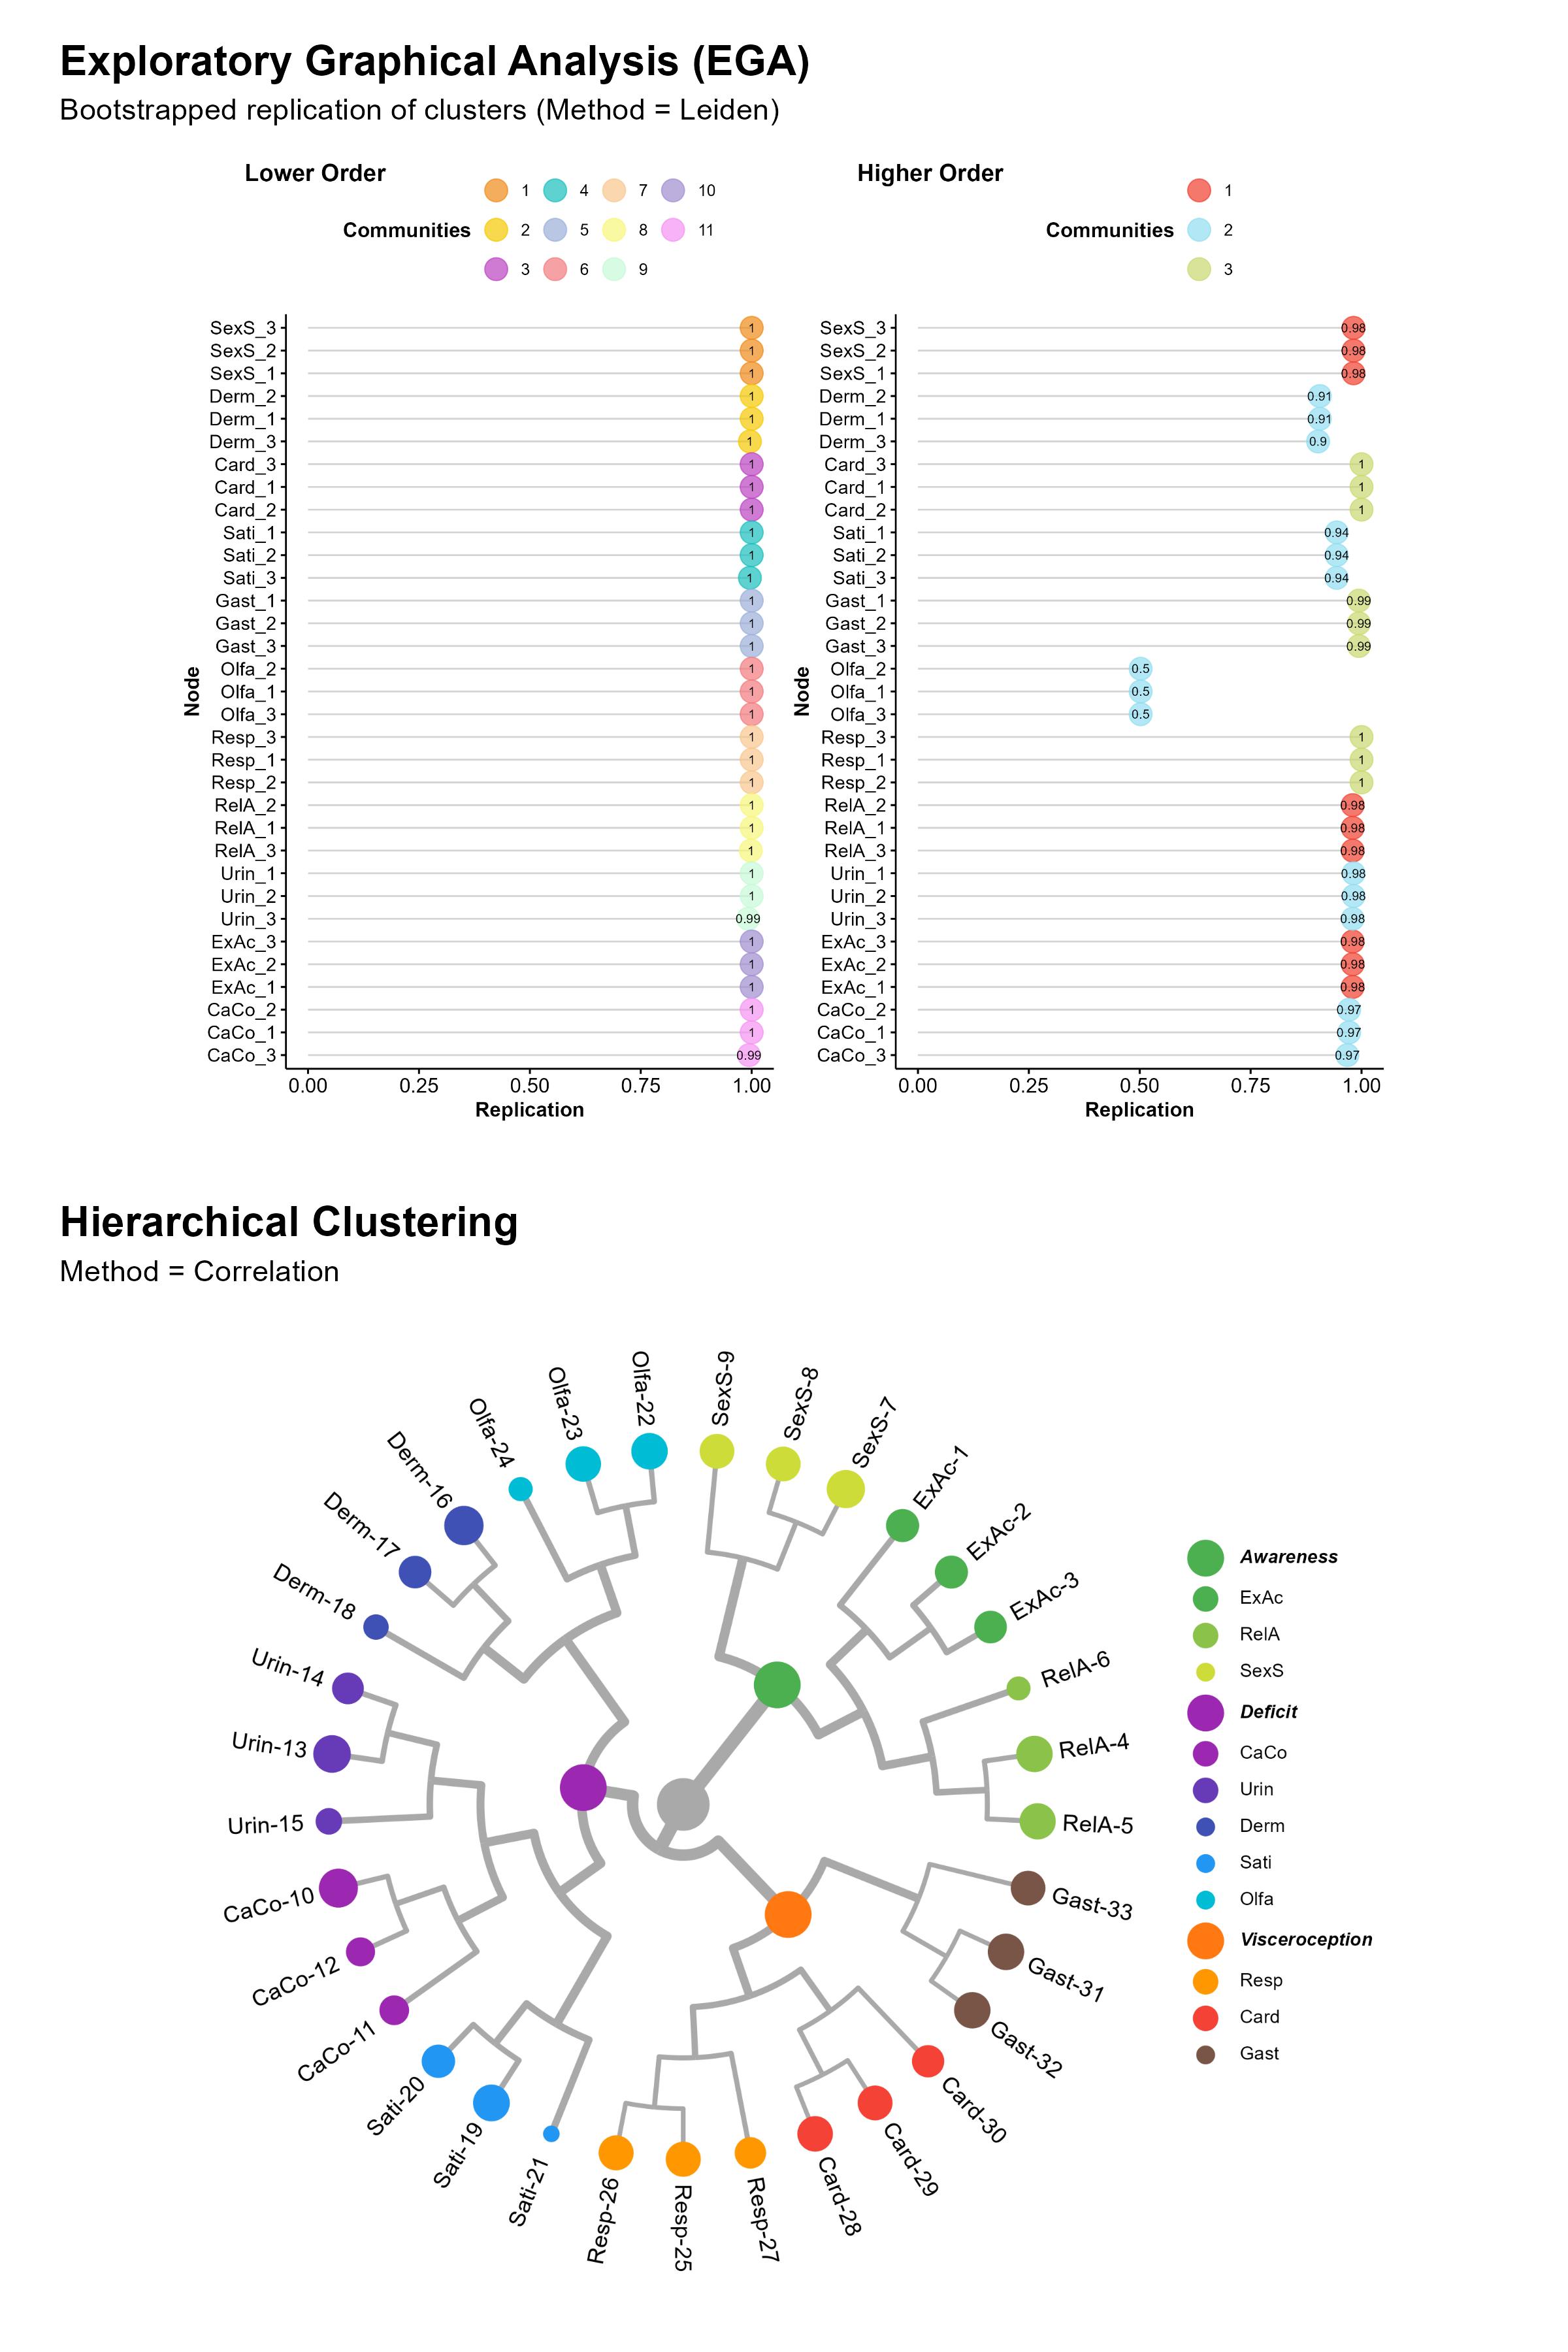
\includegraphics[width=1\linewidth,height=\textheight,keepaspectratio]{../study2/analysis/figures/fig1.png}
\end{center}

\end{figure*}

\subsection{Results}\label{results-1}

\begin{figure*}[!htbp]

{\caption{{TODO.}{\label{fig-three}}}}

\begin{center}
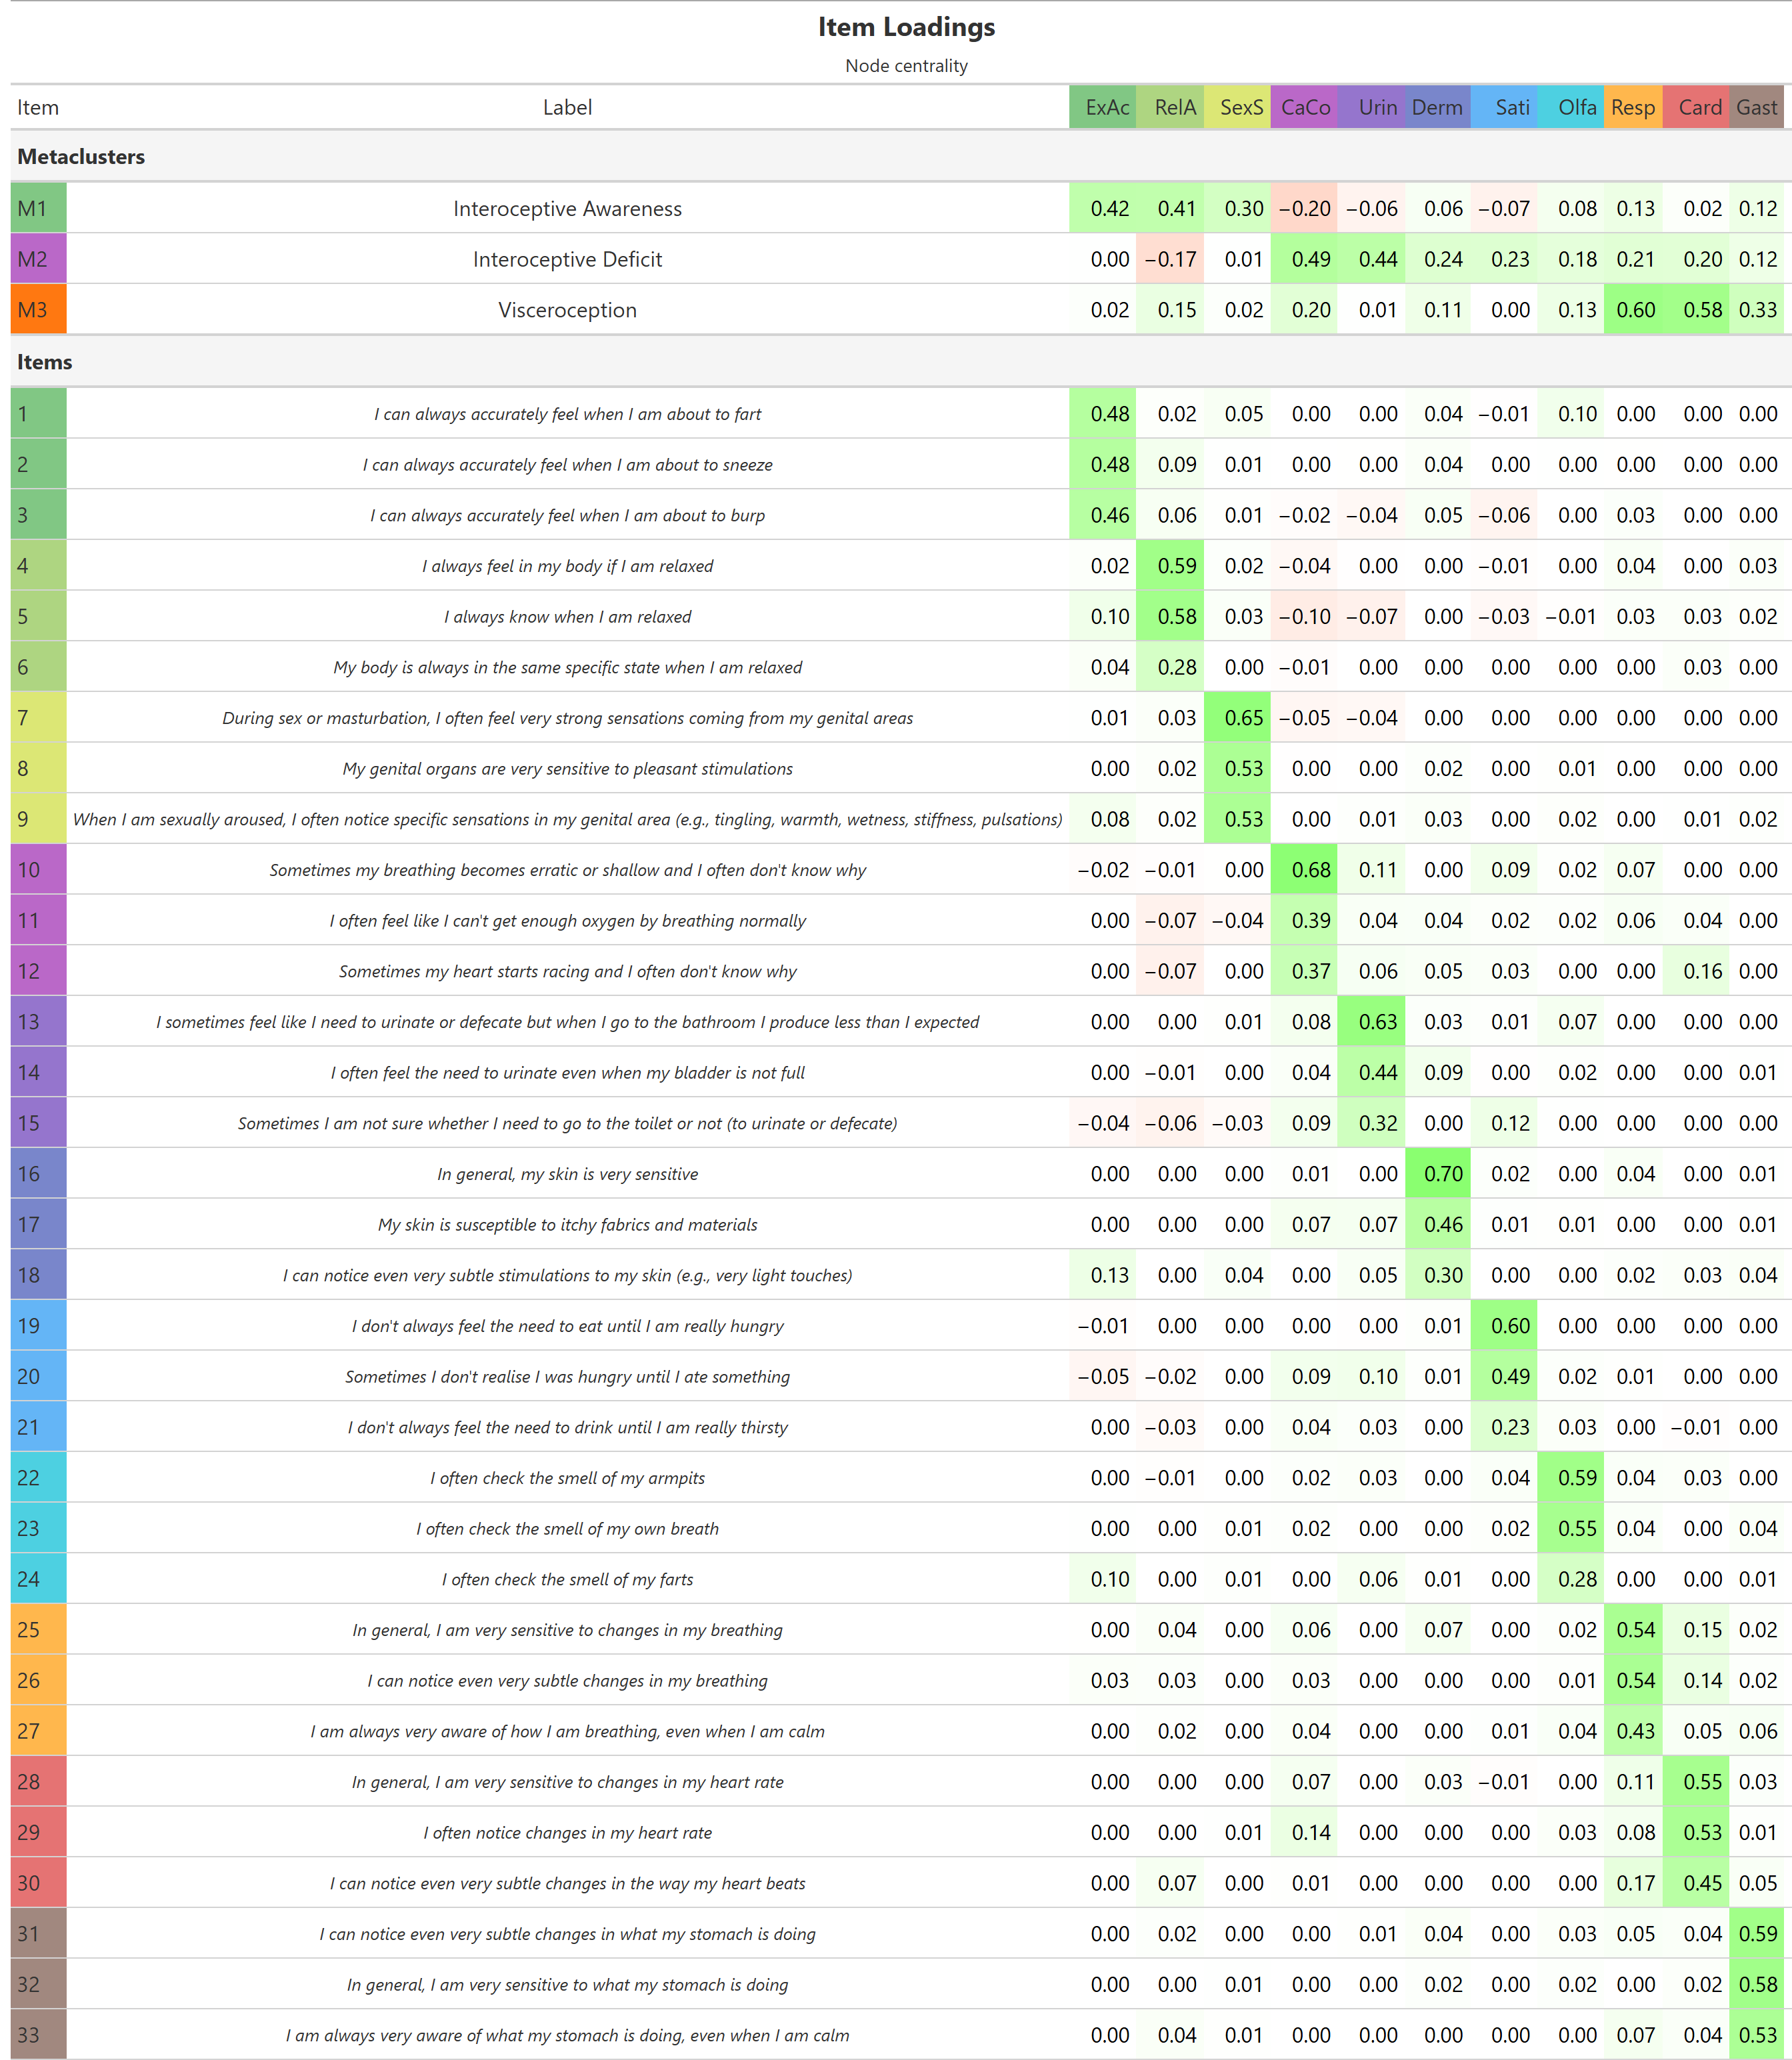
\includegraphics[width=1\linewidth,height=\textheight,keepaspectratio]{../study2/analysis/figures/table1.png}
\end{center}

\end{figure*}

\begin{figure*}[!htbp]

{\caption{{TODO.}{\label{fig-four}}}}

\begin{center}
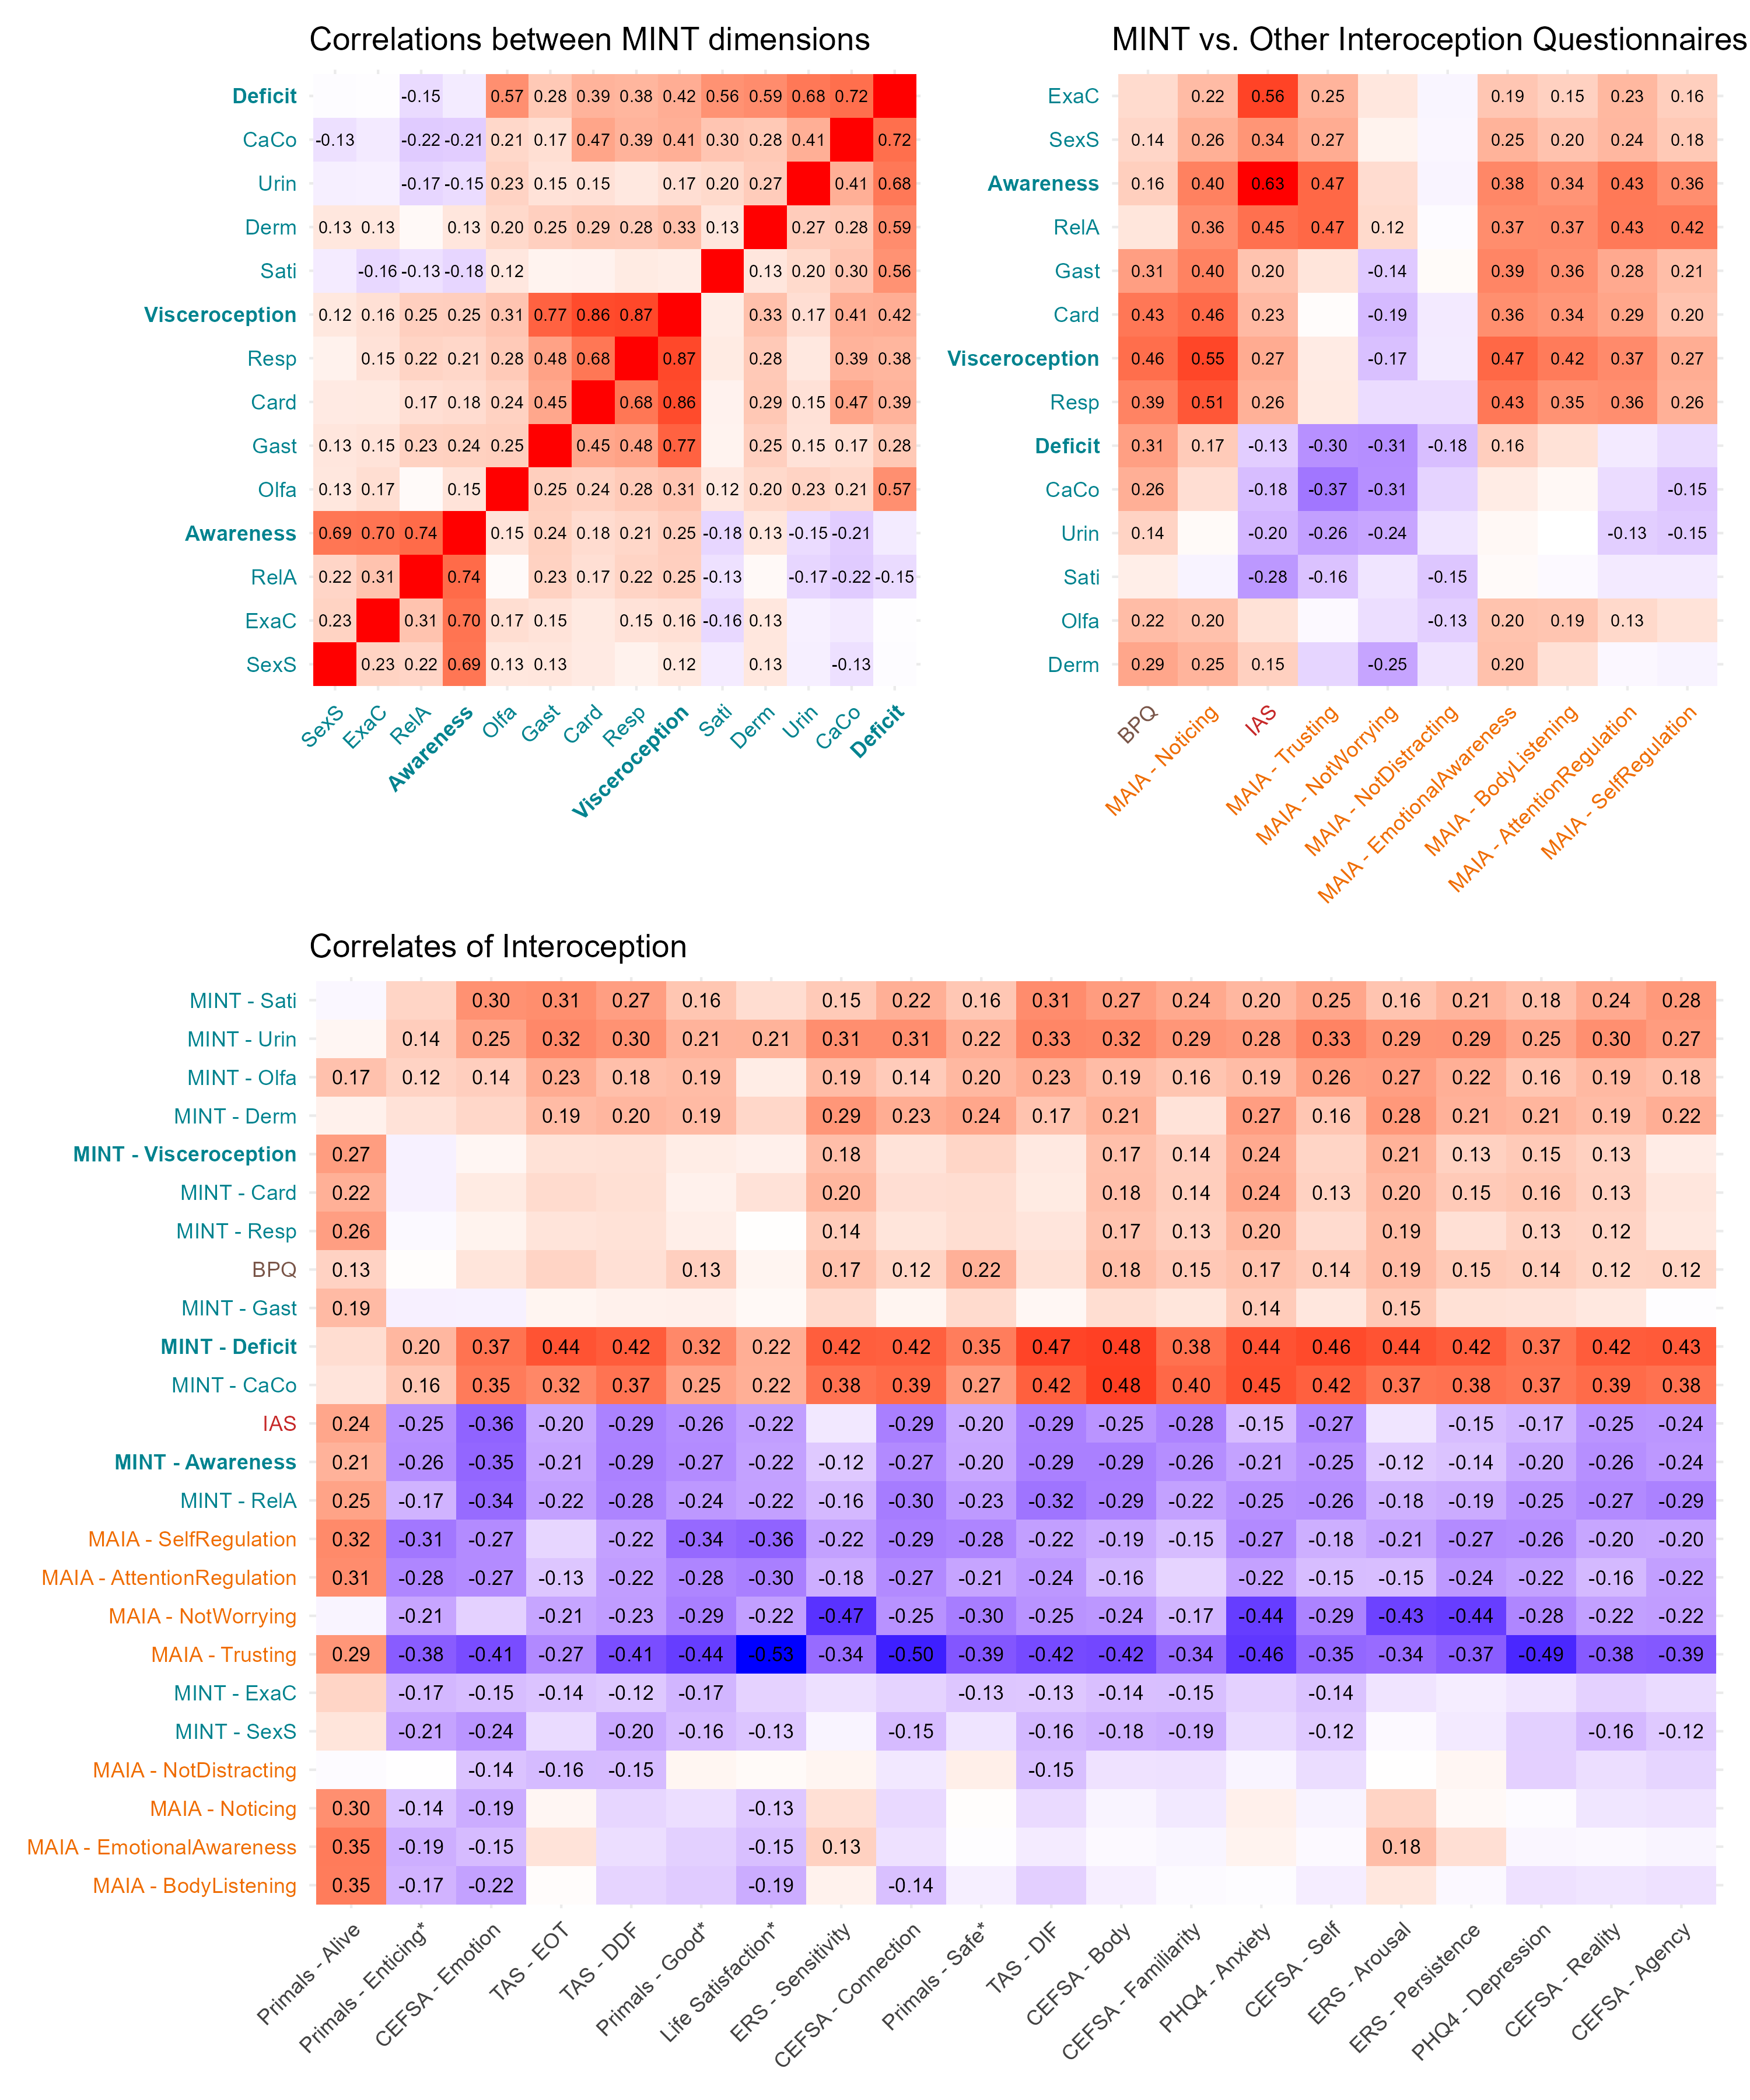
\includegraphics[width=1\linewidth,height=\textheight,keepaspectratio]{../study2/analysis/figures/fig2.png}
\end{center}

\end{figure*}

\begin{figure*}[!htbp]

{\caption{{TODO.}{\label{fig-five}}}}

\begin{center}
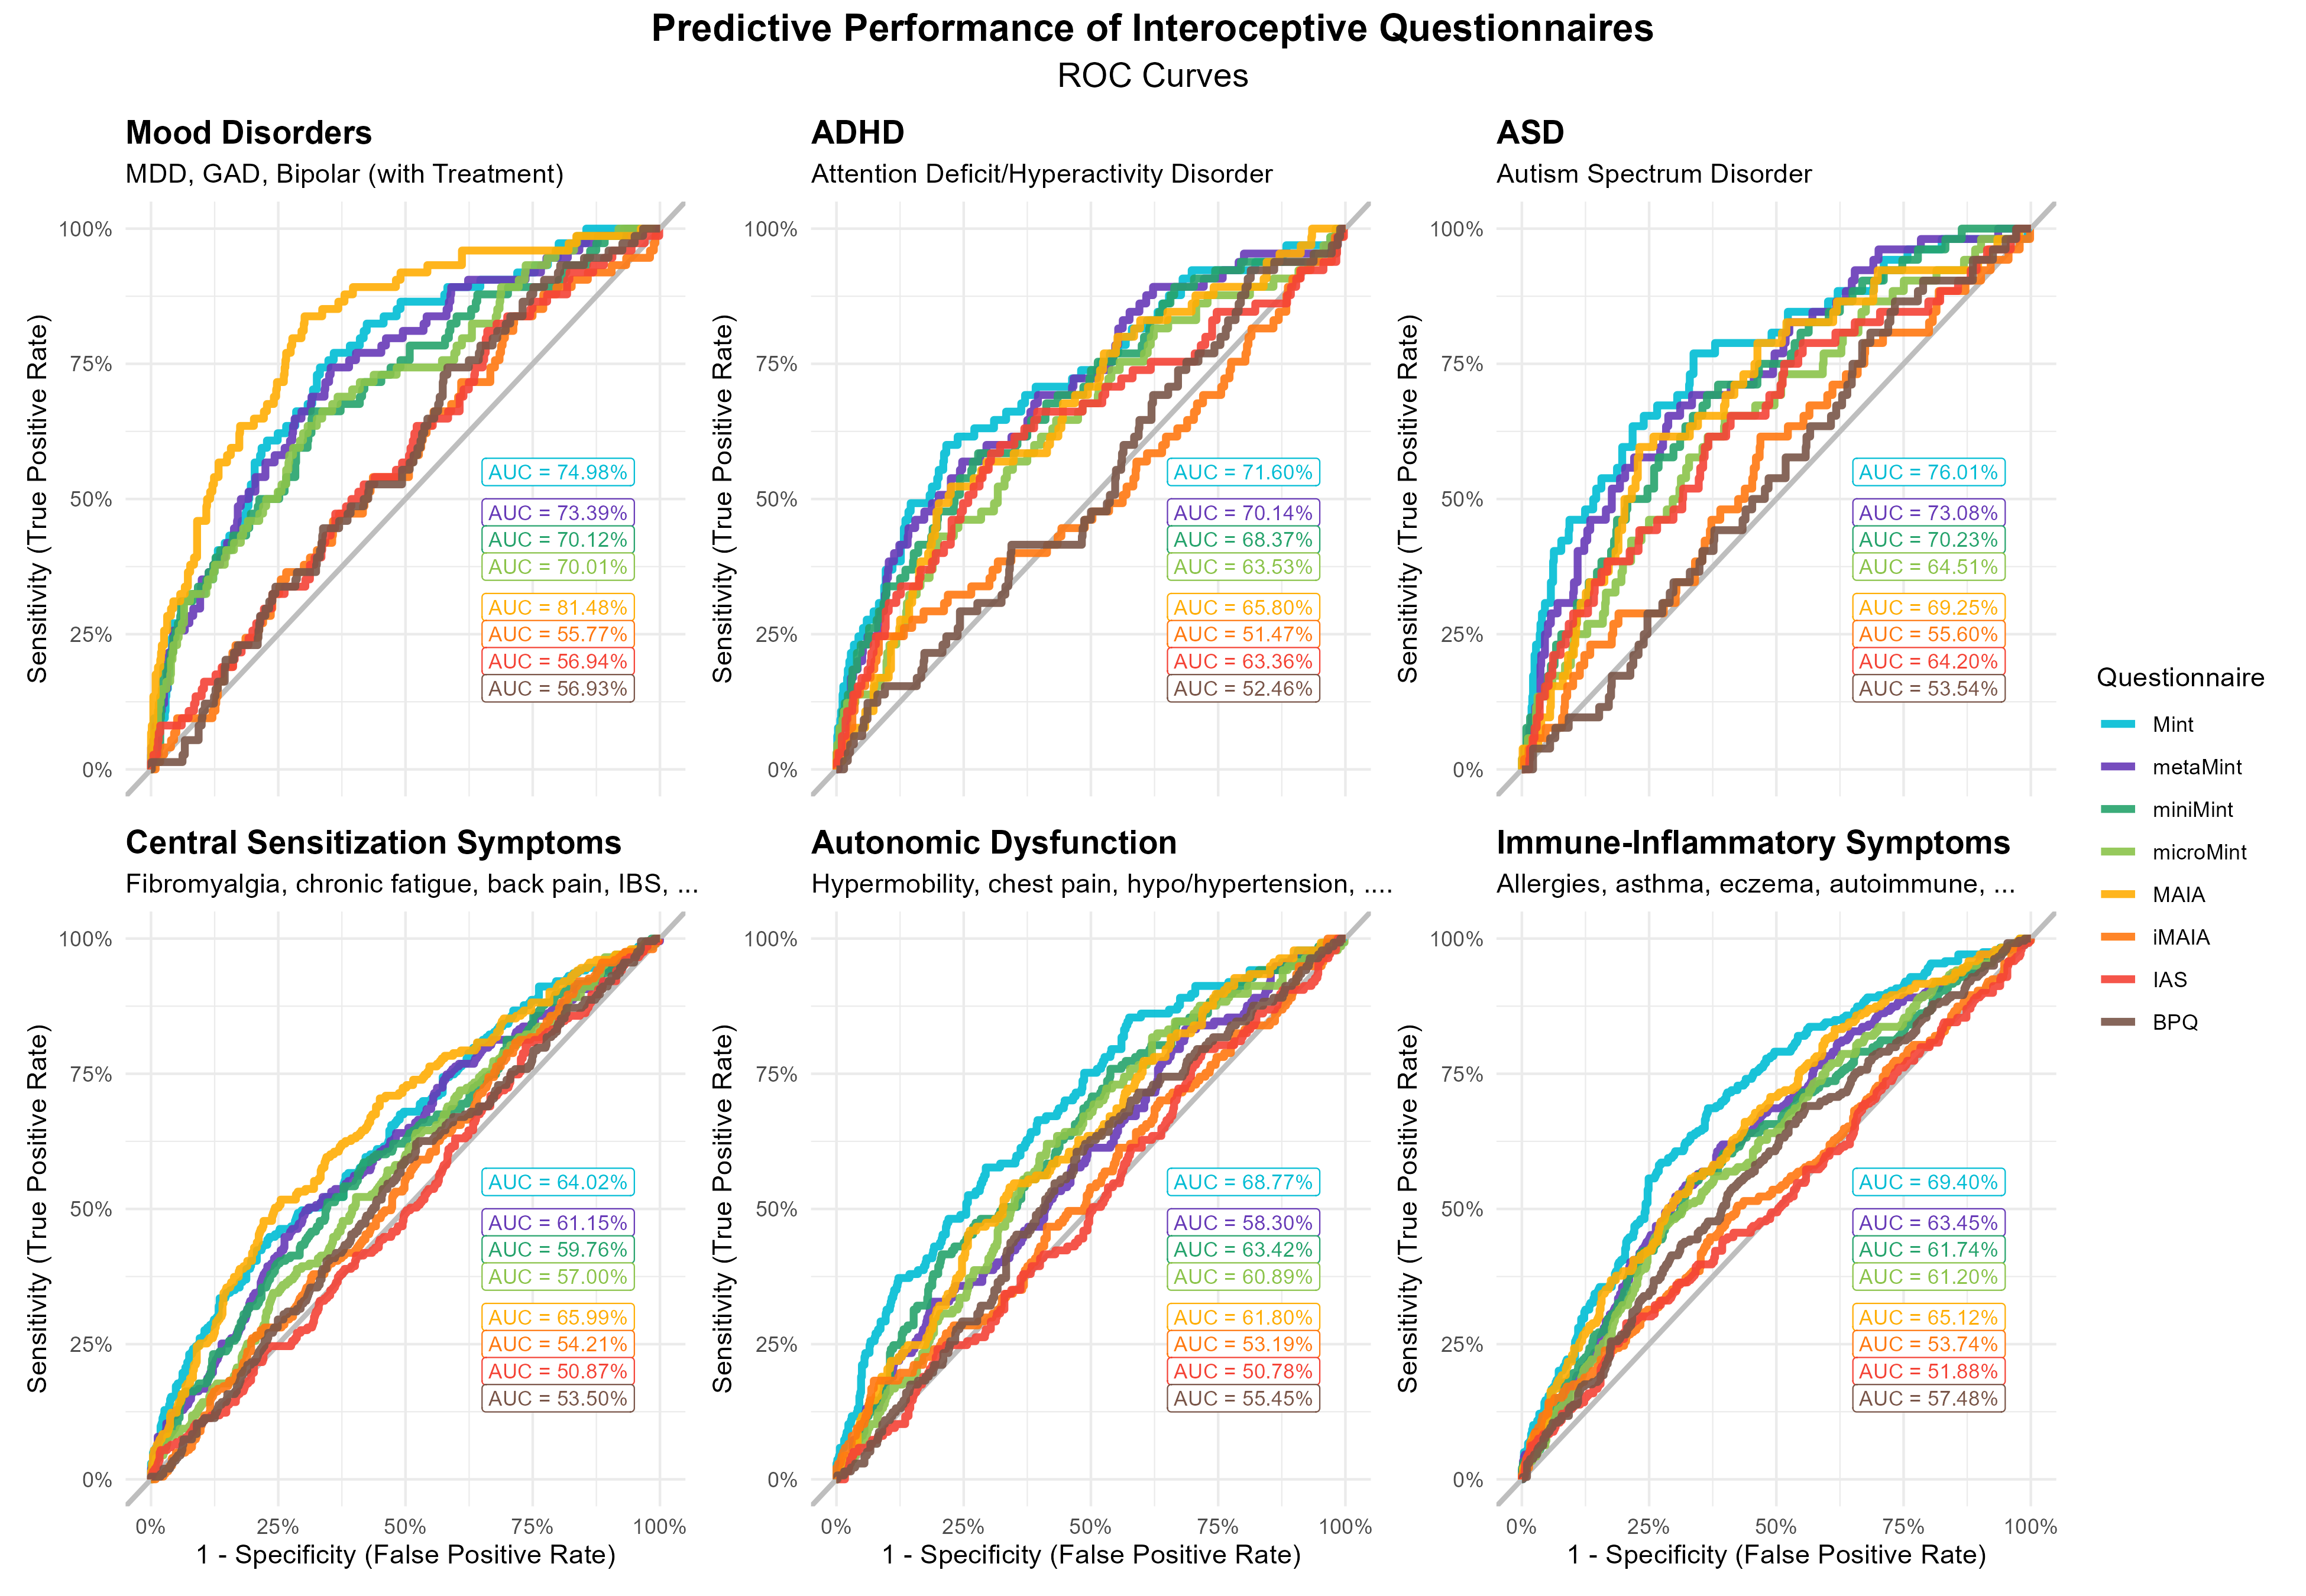
\includegraphics[width=1\linewidth,height=\textheight,keepaspectratio]{../study2/analysis/figures/fig3.png}
\end{center}

\end{figure*}

\begin{figure*}[!htbp]

{\caption{{TODO.}{\label{fig-six}}}}

\begin{center}
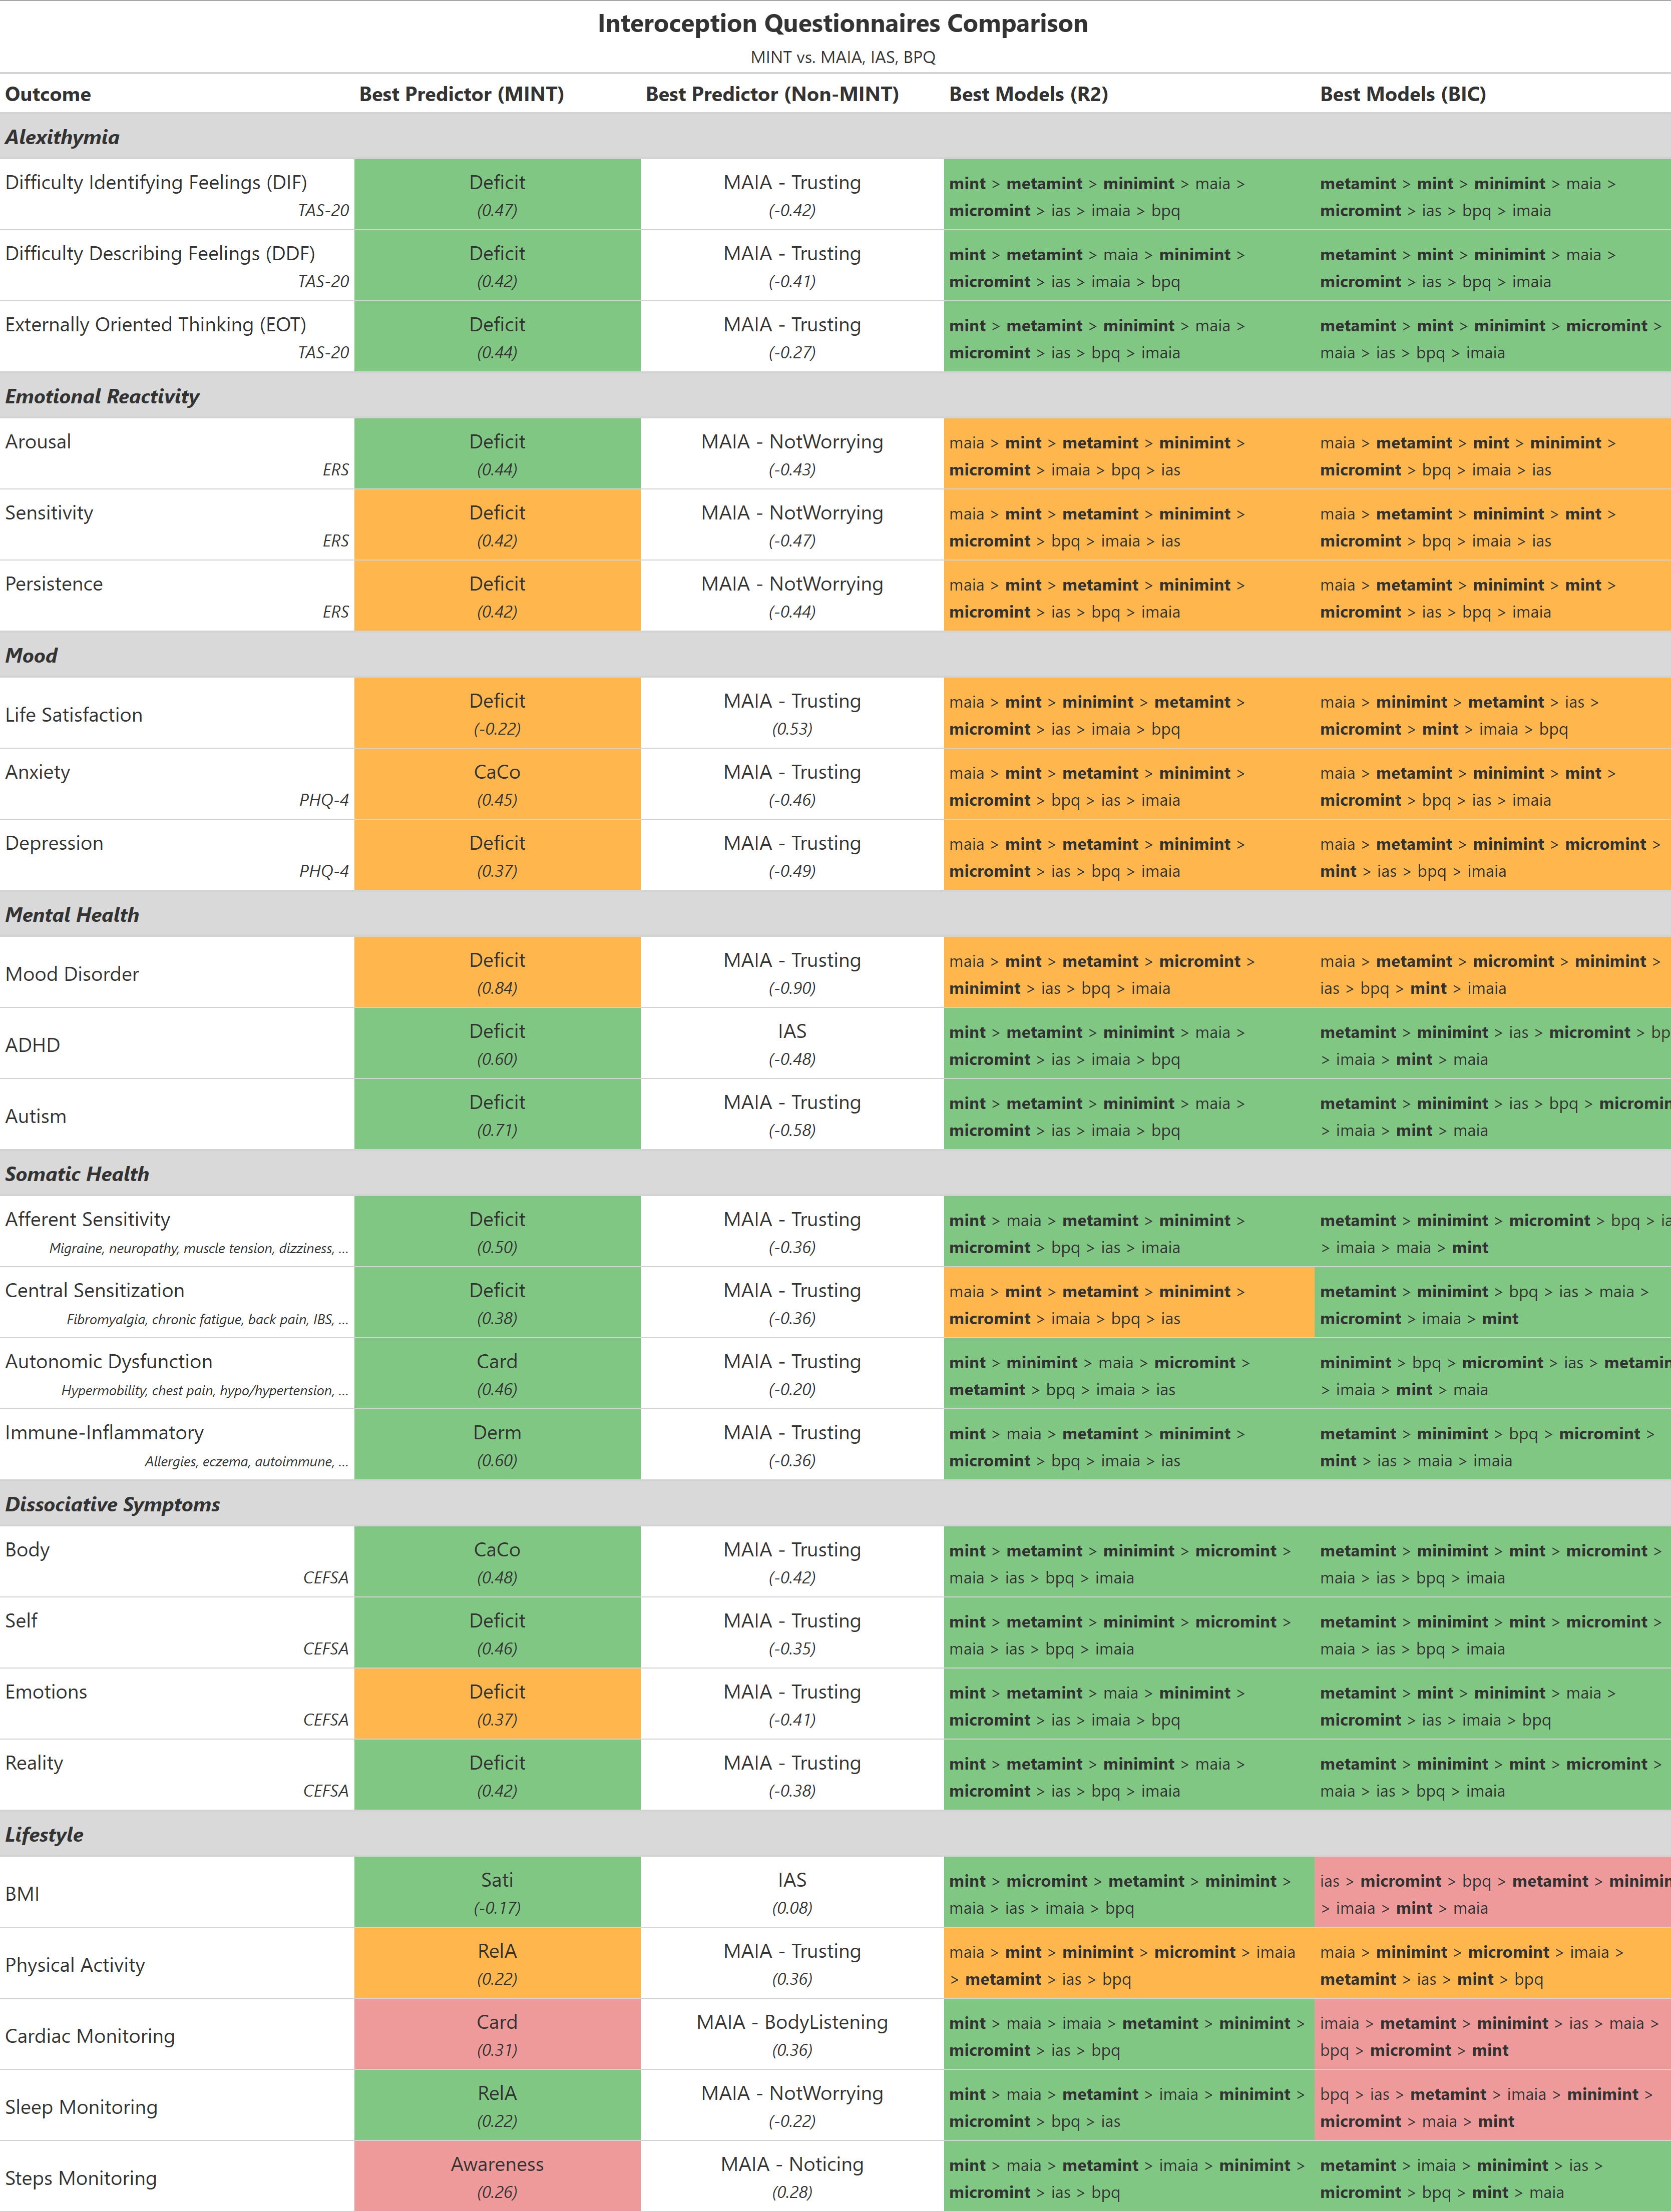
\includegraphics[width=1\linewidth,height=\textheight,keepaspectratio]{../study2/analysis/figures/table2.png}
\end{center}

\end{figure*}

\subsection{Discussion}\label{discussion-1}

\section{General Discussion}\label{general-discussion}

\section{Data Availability}\label{data-availability}

Data, code, and all materials are available at
https://github.com/RealityBending/InteroceptionScale.

\section{Acknowledgements}\label{acknowledgements}

We would like to thank the dissertation students from the University of
Sussex for their help in data collection. DM would also like to thank
\ldots{} for the motivation provided to write this paper.

\section{References}\label{references}

\phantomsection\label{refs}
\begin{CSLReferences}{1}{0}
\bibitem[\citeproctext]{ref-christensen2023unique}
Christensen, A. P., Garrido, L. E., \& Golino, H. (2023). Unique
variable analysis: A network psychometrics method to detect local
dependence. \emph{Multivariate Behavioral Research}, \emph{58}(6),
1165--1182.

\bibitem[\citeproctext]{ref-christensen2021equivalency}
Christensen, A. P., \& Golino, H. (2021). On the equivalency of factor
and network loadings. \emph{Behavior Research Methods}, \emph{53}(4),
1563--1580.

\bibitem[\citeproctext]{ref-de2015jspsych}
De Leeuw, J. R. (2015). jsPsych: A JavaScript library for creating
behavioral experiments in a web browser. \emph{Behavior Research
Methods}, \emph{47}, 1--12.

\bibitem[\citeproctext]{ref-golino2017exploratory}
Golino, H. F., \& Epskamp, S. (2017). Exploratory graph analysis: A new
approach for estimating the number of dimensions in psychological
research. \emph{PloS One}, \emph{12}(6), e0174035.

\bibitem[\citeproctext]{ref-golino2020investigating}
Golino, H., Shi, D., Christensen, A. P., Garrido, L. E., Nieto, M. D.,
Sadana, R., Thiyagarajan, J. A., \& Martinez-Molina, A. (2020).
Investigating the performance of exploratory graph analysis and
traditional techniques to identify the number of latent factors: A
simulation and tutorial. \emph{Psychological Methods}, \emph{25}(3),
292.

\bibitem[\citeproctext]{ref-indahl2018similarity}
Indahl, U. G., Næs, T., \& Liland, K. H. (2018). A similarity index for
comparing coupled matrices. \emph{Journal of Chemometrics},
\emph{32}(10), e3049.

\bibitem[\citeproctext]{ref-jimenez2023dimensionality}
Jiménez, M., Abad, F. J., Garcia-Garzon, E., Golino, H., Christensen, A.
P., \& Garrido, L. E. (2023). Dimensionality assessment in bifactor
structures with multiple general factors: A network psychometrics
approach. \emph{Psychological Methods}.

\bibitem[\citeproctext]{ref-mayer2011exploratory}
Mayer, C.-D., Lorent, J., \& Horgan, G. W. (2011). Exploratory analysis
of multiple omics datasets using the adjusted RV coefficient.
\emph{Statistical Applications in Genetics \& Molecular Biology},
\emph{10}(1).

\bibitem[\citeproctext]{ref-sibson1978studies}
Sibson, R. (1978). Studies in the robustness of multidimensional
scaling: Procrustes statistics. \emph{Journal of the Royal Statistical
Society: Series B (Methodological)}, \emph{40}(2), 234--238.

\bibitem[\citeproctext]{ref-theriault2024check}
Thériault, R., Ben-Shachar, M. S., Patil, I., Lüdecke, D., Wiernik, B.
M., \& Makowski, D. (2024). Check your outliers! An introduction to
identifying statistical outliers in r with easystats. \emph{Behavior
Research Methods}, \emph{56}(4), 4162--4172.

\end{CSLReferences}






\end{document}
